\section{METHODS}

\subsection{Digital Phantom}
Based on the fiber geometries of the digital phantom 
created for the \emph{High angular resolution diffusion imaging 
reconstruction Challenge} held in ISBI 2013 
(San Francisco, US), we simulated high resolution 
(0.5mm isotropic) T1 (TE/TR=10/1500ms) and T2 
(TE/TR=90/5000ms) images, as well as a \gls*{dmri}
(1.0mm isotropic, $b$=1200, 32 evenly-distributed 
directions, 1 \textit{b0} volume) image.
The phantom includes \gls*{wm} fiber bundles, 
\gls*{csf} and \gls*{gm}. Diffusion is modeled by a 
restricted and a hindered compartment, similar to
\cite{assaf_composite_2005}.

\subsection{Theory-based synthetic distortion}
\label{sec:distortion}
\Gls*{fmb} methodologies use a map
of the field in the scanner. More precisely, the
phase difference between two subsequent samplings
of the fieldmap. With that information, it is possible
to compute the theoretical displacement that each
voxel undergoes, the so-called \gls*{vsm}. The
most prominent feature of this \gls*{vsm} is that all
the shifts have the same orientation (parallel to the
phase-encoding direction of the \gls*{epi}) and their
magnitude and direction depend on the \gls*{epi} 
gradient increments (or \emph{blips}), and the actual
phase difference at the voxel.

In order to create a realistic distortion, we
generated a synthetic phase-difference map 
consistent with the phantom.  We defined two regions 
of smooth de-phasing (up to $0.05\pi$ rad. excursions) 
and computed the corresponding \gls*{vsm}, using the 
tools distributed with the \emph{FSL} package 
\cite{jenkinson_fsl_2012}  and
standard parameters ($\Delta$TE=2.46ms for the
fieldmap and \emph{effective dwell time} of 
0.77ms for the \gls*{epi}).

From this synthetic \gls*{vsm},
we generated
the corresponding distorted \glspl*{dwi}, in two opposed
phase-gradient encoding directions. The second simulated
``acquisition'' of the same phantom was necessary 
for evaluating \gls*{reb} methods.

Therefore, following the described strategy we generated 
a full gold-standard containing realistic T1 and T2
at high resolution, \glspl*{dwi} acquired in two
different phase encoding directions, and a ground-truth
\gls*{dwi} data, which is not available for real datasets.


\begin{figure}[thpb]
   \centering
   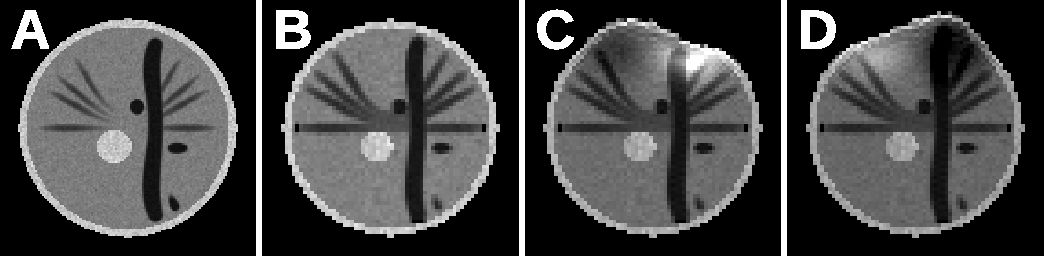
\includegraphics[width=0.95\columnwidth]{Fig01-Phantom}
   \caption{Original and distorted digital phantom.
   A) T2-weighted image; B) undistorted \textit{b0} volume;
   C, D) distorted \textit{b0} volumes with opposed phase encoding 
   directions.}
   \label{fig:label}
\end{figure}

\subsection{Correction methods}

Three out of four methods presented in \autoref{sec:intro}
were tested on the evaluation framework. 

\Gls*{fmb} correction
is essentially the same as the one used for generating the 
distortion, using the synthetic fieldmap to infer a new \gls*{vsm}.

For \Gls*{reb} correction, we made use of the implementation found 
in \emph{FSL} (\texttt{topup})
that demands for the \textit{b0} of the reverse-encoding simulation.
In this second case, the \gls*{vsm} is inferred from the differences
between the two corresponding \textit{b0}.

Finally, for evaluating \Gls*{t2b},
we fine-tuned \emph{ANTs} \cite{avants_ants:_2013},
in order to register \textit{b0} to T2. To this end, we used a
multi-resolution scheme with 3 levels of subsampling and smoothing,
mutual information metric, and symmetric diffeomorphic transform 
(\texttt{SyN}). Several configurations of kernel widths for the 
regularization smoothers were tested, and finally selected 
0.5/1.0 voxels (gradient/deformation fields, respectively) 
for its best result. Additionally, undistorted images are 
corrected for dropout using the determinant
of the Jacobian of the deformation field.

\subsection{Evaluation}

The four modules described so far (namely, phantom
deformation, \gls*{fmb} correction, \gls*{reb}
correction and \gls*{t2b} correction) were conveniently
integrated in second order workflows using
\emph{nipype} \cite{gorgolewski_nipype:_2011}.
The choice of this tool grants the reproducibility
of the experiments, among other advantages.

To evaluate the influence of
distortions on the final connectivity outcome,
an intermediate step was also implemented to
produce deterministic tractography,
using the \emph{Diffusion Toolkit} \cite{wang_diffusion_2007}.
The original phantom, one distorted version, and
the corrected instances are fed to this module.
Additionally, the original tissue probability maps
are also distorted and corrected, for computing overlap
indices.
Each tractography was restricted to its corresponding 
\gls*{wm} mask, after distortion and correction when
applied. For all the cases, we used 10 random seeds at each seeding
voxel and the seeding voxels were taken from the 
ground-truth, mimicking the usual procedure on real data
(where regions are typically mapped from the
anatomically correct T1).

The evaluation framework is completed by automated 
assessment modules. We evaluated three characteristics
of the correction methods. 
Firstly, we assessed the geometrical correctness
reporting overlap indices of three tissue
probability maps (namely \gls*{csf}, \gls*{wm},
and \gls*{gm}), weighting the average by tissue
volumes.
Secondly, to evaluate the quality of the actual 
signal dropout correction, we studied the 
similarity volume by volume computing the $\ell_1$-norm
correlation index. We report this score
on the \textit{b0} and the average of the remaining 32 
\glspl*{dwi}. Thirdly, we studied the impact on the
connectivity matrices reporting the number of
false positives (inexistent connections in the
gold-standard) and false negatives (or connections
lost).